\documentclass[10pt]{sigplanconf}

\usepackage{graphicx}
\newcommand{\code}[1]{\texttt{#1}}
\newcommand{\todo}[1]{\textbf{*** {#1} ***}}
\newcommand{\defn}[1]{\textit{#1}}

\newcommand{\startor}{\left\{ \begin{array}{ll}}
\newcommand{\stopor}{\end{array} \right.}
\newcommand{\otherwise}{\textrm{otherwise}}
\newcommand{\concept}[1]{\textit{#1}}

\newenvironment{documentation}[1]{\vspace{5pt} \noindent \texttt{#1} \nopagebreak \begin{list}{}{\leftmargin 0.7cm}\item}{\end{list}}

%% This is a trick I found on the Web for putting verbatim
%% environments inside footnotes.
\newenvironment{Footnote}{\footnote\bgroup}{\egroup}

\begin{document}

\title{Report on the Probabilistic Language Scheme}

\conferenceinfo{DLS'07,} {October 22, 2007, Montr{\'e}al, Qu{\'e}bec, Canada.}
\CopyrightYear{2007}
\copyrightdata{978-1-59593-868-8/07/0010}

%% \numberofauthors{1}

%% \author{
%% \alignauthor
%% Alexey Radul \\
%%   \affaddr{Massachusetts Institute of Technology} \\
%%   \affaddr{77 Massachusetts Avenue} \\
%%   \affaddr{Cambridge, MA 02139} \\
%%   \email{axch@mit.edu}
%% }

\authorinfo{Alexey Radul}
           {Massachusetts Institute of Technology \\ 77 Massachusetts Avenue \\ Cambrdige, MA 02139}
           {axch@mit.edu}

\maketitle

\begin{abstract}
Reasoning with probabilistic models is a widespread and
successful technique in areas ranging from computer vision, to natural
language processing, to bioinformatics.  Currently, these reasoning
systems are either coded from scratch in general-purpose languages or
use formalisms such as Bayesian networks that have limited expressive
power.  In both cases, the resulting systems are difficult to modify,
maintain, compose, and interoperate with.  This work presents Probabilistic
Scheme, an embedding of probabilistic computation into Scheme.  This
gives programmers an expressive language for implementing modular
probabilistic models that integrate naturally with the rest of Scheme.
\end{abstract}

\category{D.3.3}{Programming Languages}{Language Constructs and Features}
\terms Algorithms, Design, Languages
\keywords Scheme, embedding, probability

\section{Introduction}
\label{introduction}

Some of the most challenging tasks faced by computers today involve
drawing conclusions from noisy or ambiguous data.  These tasks range
from deciding whether an email message is spam based on the words it
contains~\cite{sahami1998baf}, to predicting whether a piece of ground
is safe to drive on based on camera and laser range-finder
readings~\cite{thrun2006pta}, to discovering patterns of gene
expression based on microarray data~\cite{segal2001rpm}.
Probabilistic modeling has become the technique of choice for tackling
many of these tasks (as illustrated by the papers just cited).
Probability theory provides a well-understood mathematical framework
for combining multiple sources of evidence, but the computational
tools available to programmers wishing to avail themselves of it are
limited.

Probabilistic Scheme is a library for implementing probability models
in Scheme.  Probabilistic Scheme deals with models of phenomena in
arbitrarily structured but discrete and countable possibility spaces.
The main contributions of Probabilistic Scheme are that it is an 
embedding of probabilistic computation into a general-purpose
programming language; that it offers anytime approximation with
provable upper and lower bounds via restartable partial search; and
that it can be implemented with continuations, without using a
meta-circular evaluator, so that it can interoperate seamlessly
with much of the rest of the language.

The central concept in Probabilistic Scheme is
that of a probability distribution.  A
probability distribution, in this context, is a belief about the value
that an expression could have when evaluated in some environment.
Suppose, for example, that I were about to roll a mathematically
perfect six-sided die.  Then you should believe that each of the six
faces is equally likely to come up as the final result, and no other
results are possible.  This belief is a \defn{probability
distribution}, which assigns probability one-sixth to each of the
faces of the die.  Suppose, then, that you asked me the parity of the
result and I informed you that the number rolled on the die were odd.
Then, assuming you had no doubts about my perceptiveness or veracity,
your belief about the result of the roll would change to one that
assigned probability one-third to each of the faces with odd numbers,
and zero to the others.

Probabilistic Scheme permits one to represent
such beliefs, from the simple to the complex; to compute their
transformations; and to extract definite, quantitative information
from them.  As a preview, the beliefs in the preceding paragraph can
be represented as follows
\begin{verbatim}
(define die-roll-distribution
  (make-discrete-distribution
   '(1 1/6) '(2 1/6) '(3 1/6)
   '(4 1/6) '(5 1/6) '(6 1/6)))

(define odd-die-roll-distribution
  (conditional-distribution
   die-roll-distribution odd?))

(distribution/determine!
 odd-die-roll-distribution)
(distribution/datum-probability
 odd-die-roll-distribution 1)
;Value: 1/3
\end{verbatim}

Conceptually, distributions in Probabilistic Scheme are lists of the
possibilities, and the probabilities assigned to them.  If some object
does not appear in the list, its probability is zero.  To permit large
(or infinite) distributions which are not needed in their entirety at
any one time, this is actually a stream\footnote{A stream is a
(possibly infinite) list whose actual construction has been delayed so
that it is only ever computed as far as any client requests~\cite{sicp}.} of
possibilities.  The representation of probability distributions will be
further detailed in Section~\ref{querying} and
Section~\ref{implementation}.

Probabilistic Scheme offers two ``languages'' for creating and
transforming distributions.  There is a language for constructing
probability distributions by writing nondeterministic
Scheme programs, described in Section~\ref{implicit}.
There is also a language for explicitly
creating and manipulating objects that represent probability
distributions, described in Section~\ref{explicit}.  
The explicit language is easier to think about,
because there are no weird control structures or strange
nondeterministic programs, but the nondeterministic language is better suited
to defining complex distributions, because it makes the structure of
the distribution much clearer and its expression much more natural.

Probabilistic Scheme also offers a language for querying distributions
to extract definite information from them.  This turns out to be
somewhat nontrivial, and is discussed in Section~\ref{querying}.  We
discuss our implementation of these languages in
Section~\ref{implementation}, with a detailed walkthrough in 
Section~\ref{sec:walkthrough}, exemplify some unusual distributions
definable in Probabilistic Scheme
in Section~\ref{examples}, and summarize
in Section~\ref{discussion}.  First, though, some background,
in Section~\ref{background}.

\section{Background}
\label{background}

Bayesian networks have been a mainstay of probabilistic modeling since
the late 1980s,
e.g.~\cite{russell1995aim}.  They are a wonderful basic tool, and well
implemented by off-the-shelf inference packages such as
BUGS~\cite{spiegelhalter1994bbi}, but they are not very good at
capturing the structure present in a domain.  Recent work has moved in
the direction of increased structure, for instance capturing
relational structure as in~\cite{koller1998pfb}
and~\cite{friedman1999lpr}, or first-order logical structure as
in~\cite{milch2005bpm}.  

Probabilistic Scheme goes beyond this work, in the sense that programs
in a general-purpose programming language are as structured as it is
possible to be.  The modeler is not constrained to expressing the
model as a finite list of individual variables, as in a standard Bayes
net; nor as a fixed object graph with known interobject links, as in
standard relational models; nor as a fixed set of formulas that are
only first order.  Any construct expressible in Scheme, be it objects,
functions, recursion, higher-order routines, etc can be subject to
uncertainty and reasoned about.

The closest modern relative to Probabilistic Scheme is a stochastic
programming language based on OCaml, called IBAL~\cite{pfeffer01ibal}.
Probabilistic Scheme differs from IBAL in being an embedding of
inference into an existing programming language, rather than a
new programming language in its own right, permitting Probabilistic Scheme
to benefit from all of the extant Scheme constructs.
Another piece of related work is by Ramsey and Pfeffer~\cite{ramsey2002slc},
who explore denotational semantics for a form of stochastic lambda
calculus similar to the stochastic sublanguage of Probabilistic
Scheme.  We take a more operational approach to semantics in the
present work.
The stochastic
sublanguage of Probabilistic Scheme owes a great
intellectual debt to McCarthy's \code{amb} operator (see,
e.g.~\cite{mccarthy1963bmt}, \cite{sicp}).

\section{Stochastic Language}
\label{implicit}

Probabilistic Scheme embeds probabilistic computation by allowing
Scheme expressions to have uncertain values, and maintaining an
implicit probability distribution over what those values might be.
The primitives for handling implicit distributions are
\begin{itemize}
\item \code{discrete-select} introduces uncertainty
\item \code{observe!}\ constrains the implicit distribution
\item \code{stochastic-thunk->distribution} encloses a nondeterministic
computation and returns the implicit distribution explicitly.
\end{itemize}

We now discuss each of these primitives in detail.

\begin{documentation}{(discrete-select possibility ...)}
Takes any number of literal two-element lists representing object-probability
pairs.
Returns one of the objects, implicitly distributed according to the
distribution specified by the probabilities, which are expected to
sum to 1.  The evaluation of each object is deferred until it
needs to be returned.
\end{documentation}

As expressions combine, their implicit distributions transform according
to the rules of probability theory.  For example,
we can
\begin{verbatim}
(define (roll-die)
  (discrete-select (1 1/6) (2 1/6) (3 1/6)
                   (4 1/6) (5 1/6) (6 1/6)))
\end{verbatim}
Then every call to the \code{(roll-die)} function will independently 
return one of
the numbers from 1 through 6, implicitly uniformly distributed.  In
that case, the expression \code{(cons (roll-die) (roll-die))} returns
one of the 36 cons cells that have one of those numbers in the car
slot and one in the cdr slot, also implicitly uniformly distributed.
The expression \code{(+ (roll-die) (roll-die))} will return one of the
numbers from 2 through 12, implictly distributed according to the
probability of getting that sum when rolling two fair six sided dice.
These rules of combination allow one to define arbitrarily complex
distributions over arbitrarily structured objects.

\begin{documentation}{(observe!\ boolean)}
Modifies the current implicit distribution by conditioning
it on the argument being true.  Returns an unspecified value.
\end{documentation}

Consider, for example, the expression
\begin{verbatim}
(let ((face (roll-die))) ;; Line 1
  (observe! (> face 2))  ;; Line 2
  face)                  ;; Line 3
\end{verbatim}
In line 1, the expression \code{(roll-die)} returns one of the numbers
from 1 through 6, implicitly unformly distributed.  \code{Let} then
binds it to the name \code{face}, whose value is then implicitly
uniformly distributed over 1 through 6.  The expression \code{(> face
2)} on line 2 has one of the values \code{\#t}, \code{\#f}, implicitly
distributed as 2/3 for \code{\#t} and 1/3 for \code{\#f}.
\code{Observe!}\ modifies this implicit distribution to require
\code{\#t}.  This modifies the implicit distribution for \code{face}
to be consistent with \code{(> face 2)} returning \code{\#t}, that is
it conditions $p(\code{face})$ on \code{(> face 2)}.  The
distribution of return values from this whole \code{let} form is then
$p(\code{face}|\code{(> face 2)})$, in other words uniform over the
numbers from 3 through 6.

\begin{documentation}{(stochastic-thunk->distribution thunk)}
Returns, as an explicit probability distribution, the implicit
distribution over the possible return values of the given thunk
(nullary procedure).
\end{documentation}

For example,
\code{(stochastic-thunk->distribution roll-die)} would return an
explicit distribution object that represented the
distribution that assigns equal mass to the numbers $1, 2, \ldots, 6$.
\code{Stochastic-thunk->distribution} captures and contains the
nondeterminism occurring inside its argument thunk and perfectly
deterministically returns an object representing a probability
distribution.\begin{Footnote}Nondeterministic computations can be nested:
\begin{verbatim}
(stochastic-thunk->distribution
 (lambda ()
   (discrete-select
    ((stochastic-thunk->distribution
      (lambda ()
       (discrete-select ('heads 1/2)
                        ('tails 1/2)))) 1/5)
    ((stochastic-thunk->distribution
      (lambda ()
       (discrete-select
        (1 1/3) (2 1/3) (3 1/3)))) 4/5))))
\end{verbatim}
will return an explicit probability distribution weighted 1/5 to 4/5,
whose two data are two different explicit probability
distributions.\end{Footnote}

One way to think of the semantics of the stochastic language is to
imagine a possible implementation by rejection sampling.  One could
implement rejection sampling for this stochastic language by having
\code{discrete-select} just use a random number generator, having
\code{observe!}\ raise a distinguished exception if its argument
is false, and having \code{stochastic-thunk->distribution} run its
thunk many times, recording every successful return as a sample, and
throwing away runs that raised the exception.  In
the limit of running the thunk an infinite number of times, the
samples thus produced would constitute the distribution defined
by such a program.

The actual implementation systematically searches the space of
possibilities instead.  The choice points introduced by
\code{discrete-select} define a tree of possible computations.
Computations that successfully return from the thunk given to
\code{stochastic-thunk->distribution} result in acceptable
possibilities, whereas computations that lead to \code{(observe! \#f)}
result in impossibilities.  The details of the implementation are
discussed in Section~\ref{implementation}, but they have one important
effect on the specification: Since searching the space of
possibilities may entail calls to \code{discrete-select} returning
fewer or more times than once, the results of intermixing
\code{discrete-select} with side effects are unspecified.

\section{Explicit Distribution Language}
\label{explicit}

As well as specifying distributions with nondeterministic thunks given
to \code{stochastic-thunk->distribution}, one can create and operate
on explicit probability distributions directly.  The
primitives\footnote{Actually, \code{distribution-select} is enough for
everything, because these operations are readily implementable by
falling through to the stochastic language.  This list is primitive in
the sense that these operations are a sufficient base even without
reference to the stochastic language.} for handling explicit
distributions are
\begin{itemize}
\item \code{make-discrete-distribution} creates an explicit probability
distribution from a list of possibilities
\item \code{dependent-product} combines two distributions
\item \code{conditional-distribution} transforms a distribution
by conditioning it on a predicate
\item \code{distribution-select} makes an explicit distribution
implicit
\end{itemize}

\begin{documentation}{(make-discrete-distribution possibility ...)}
Interprets each possibility argument as a two-element list of an object
and its probability.  Returns the probability distribution that assigns
those probabilities to those objects, and zero to all others.
Expects the set of possibilities to be normalized, i.e.\ for the
given probabilities to sum to 1.
\end{documentation}

\begin{documentation}{(dependent-product \\ \mbox{} distribution function combiner)}
A distribution $p(y|X)$ that depends on the value of some variable
$X$ can be represented as a function of $X$ that, when given any
particular value $x$, returns the distribution $p(y|X=x)$.  Given a
distribution $p(x)$ and such a function \code{(lambda (x)
p(y|X=x))}, \code{dependent-product} returns the distribution
$p(x,y) = p(x)p(y|X=x)$.  Instead of
trying to represent a distribution over multiple values,
\code{dependent-product} takes a combiner to apply to the values $x$
and $y$, to return $p(\code{(combiner x y)})$.  An oft-useful
combiner is \code{cons}, though the right summation will happen
if the combiner maps multiple pairs to the same combined value.
\end{documentation}

\begin{documentation}{(conditional-distribution \\ \mbox{} distribution predicate)}
Given a distribution $p(x)$ and a predicate $A(x)$, returns the distribution
over $x$'es that satisfy the predicate, which
is given by
\[ p(x|A(x)) = \startor
p(x) / p(A) &    \textrm{if $A(x)$ is true} \\
0 &              \textrm{if $A(x)$ is false} \\
\stopor \]
where $p(A)$ is the probability that $A$ is true.  Since the $x$'es are
mutually exclusive and exhaustive, we know that
\[ p(A) = \sum_{x:A(x)} p(x). \]
\end{documentation}

The behavior of the system is unspecified if the predicate $A(x)$ is
impossible to satisfy.  The present implementation
will either enter an infinite loop if the underlying
stream is infinite, or fail with an error if it is
finite.

\begin{documentation}{(distribution-select distribution)}
Returns one of the possible values from the given explicit
distribution, implicitly distributed according thereto.
\end{documentation}

For example, \code{roll-die}, above, could have been defined as
\begin{verbatim}
(define (roll-die)
  (distribution-select
   (make-discrete-distribution
    '(1 1/6) '(2 1/6) '(3 1/6)
    '(4 1/6) '(5 1/6) '(6 1/6))))
\end{verbatim}

\section{Querying Distributions}
\label{querying}

Probability distributions are occasionally infinite, as for instance a
Poisson distribution over the integers, and often
technically finite but large enough that we do not wish to compute
them fully, as for instance a distribution over the possible parses
of some sentence.  Exact answers to questions about the probabilities
of things in such distributions are therefore unobtainable in general,
and we must turn to approximations.  Probabilistic Scheme offers
an API that leads to an anytime approximation\footnote{Anytime 
approximation is a buzzword meaning that the client can choose how much
time to invest in a computation and receive the best answer the 
system can give in the allotted time.} strategy, and has the 
advantage of giving exact upper and lower bounds on its approximate
answers.

Probabilistic Scheme achieves anytime approximation with a lazy
representation of distributions.  On initial creation, a distribution
is a completely unforced stream of possibilities, each of which names
a value and some amount of probability that the distribution assigns
to it.  On user request, this internal stream can be (partially)
forced, whereupon the distribution object caches the assignments that
came out of it.  Therefore, at any one time, a distribution will have
some cache of the possibilities that came out of the stream so far,
which it can use to answer questions, and an upper bound on the amount
of probability remaining in the rest of the stream.

It is convenient to permit the internal stream of a distribution
to emit impossibilities as well as possibilities.  An impossibility
has the meaning that some amount of probability ``vanishes,'' in
which case the distribution object implicitly renormalizes.  This
happens, for instance, if some \code{observe!}\ statement forces some condition
that otherwise had some probability of being false.
In the sequel, we use the word 'density' to refer to the actual
numbers in the possibilities and impossibilities, and the word 'mass'
to refer to probabilities derived from them by normalization.
It is an invariant of Probabilistic Scheme that
the total density in the possibilities and impossibilities in
any stream from which a distribution is made is 1.

\subsection{Questions}

The following queries can be applied to explicit probability
distributions without further forcing:

\begin{documentation}{(distribution?\ thing)}
Returns \code{\#t} if the given thing is an object explicitly
representing a probability distribution, and \code{\#f} otherwise.
\end{documentation}

\begin{documentation}{(distribution/determined?\ distribution)}
Returns whether the given distribution object has already been fully
determined, as opposed to having more computation it could do to
further refine its internal representation of the distribution it
represents.
\end{documentation}

\begin{documentation}{(distribution/undetermined-mass distribution)}
Returns the amount of probability mass that remains in the unforced
segment of the internal possibility stream in this distribution.
\end{documentation}

\begin{documentation}{(distribution/datum-min-probability \\ \mbox{} distribution datum) \\
(distribution/datum-max-probability \\ \mbox{} distribution datum) \\
(distribution/datum-probability \\ \mbox{} distribution datum)}
Return bounds on the probability that the given datum could have in
this distribution.  The minimum value will be realized if all the
remaining undetermined mass goes to other data.  The maximum value
will be realized if all the remaining undetermined mass goes to this
datum.  The unqualified function will signal an error if any
undetermined mass remains, because then the probability of the
datum is as yet unknown.
\end{documentation}

\subsection{Forcing}

The following functions cause explicit probability distribution
objects to perform more of their computations:

\begin{documentation}{(distribution/refine!\ distribution)}
Runs the computation in the given distribution for the smallest
detectable increment, which is either until a possibility is
discovered or until some undetermined mass is lost to an
impossibility.  If the former comes to pass, the \code{min-probability} of the
datum of the discovered possibility increases, and the
\code{max-probability} of every other datum decreases.  In the latter
case, the \code{min-probability} of every thus far discovered datum increases
and the \code{max-probability} of every datum decreases, unless there
could be only one datum.  The \code{undetermined-mass} decreases
unless no data have yet been found, in which case it remains 1.

If the computation has been finished, i.e.\ no
undetermined mass remains, \code{distribution/refine!}\ does nothing
and returns \code{\#f}.  If \code{distribution/refine!}\ did
anything, it returns \code{\#t}.  Higher-level forcing functions can
be built by iterating \code{distribution/refine!}\ for some desired
amount of time or until some desired condition has been met.
\end{documentation}

\begin{documentation}{(distribution/determine!\ distribution)}
Runs the computation in the given distribution all the way to the end.
This is useful primarily for testing.
\end{documentation}

\begin{documentation}{(distribution->density-stream distribution)}
Returns a stream of the possibilities in the given distribution.  The
stream is permitted to contain impossibilities and repeated data at
the discretion of the underlying implementation.  This is an effective
way to iterate over all the possibilities of a distribution, without
requiring it to compute any beyond those that the client deems
interesting.  The returned stream starts with values from the
distribution's cache, but will begin to force the distribution's
internal stream when necessary (which forcing will be correctly cached
for future access).
\end{documentation}

\section{Implementation}
\label{implementation}

We first discuss our implementation of the explicit probability
distribution objects, and then proceed to the implementation of the
stochastic language.  We present a detailed example of the workings of
the present implementation Probabilistic Scheme in
Section~\ref{sec:walkthrough}.

\subsection{Distributions}

As mentioned in Section~\ref{querying}, a probability distribution is
fundamentally a stream of possibilities and impossibilities.  A
possibility assigns some density to some particular datum, and an
impossibility asserts that some density ``disappears'', and the rest
should be renormalized to account for that.\footnote{We use the word
\concept{density} here instead of probability to emphasize the need
for normalization.}  Our distribution
objects do not perform the renormalization eagerly, but instead track
the total density of the impossibilities, and perform the
renormalization on the fly as clients ask for the probabilities of
various data.

A distribution is then a record containing four components:
\begin{itemize}
 \item a lazy stream of the possibilities and impossibilities
   that form the distribution;
 \item a hash table mapping the data that we have encountered so far
   to their respective densities;
 \item a measure of how much density remains in
   the stream, the \concept{undetermined density}; and
 \item the total density of the impossibilities we have encountered, the
   \concept{discarded density}.
\end{itemize}

The probability of some datum in a given distribution is its
 normalized density --- density divided by the distribution's
 \concept{normalization constant}, which is one minus the density that
 has been discarded due to impossibilities.
If a distribution has not been completely determined, i.e.\ the
 possibility stream has not been exhausted, the probability of any
 datum is not completely certain.
It can, however, be bounded from above by assuming that all the
 undetermined density will go to this datum, and from below by
 assuming it will all go to other data.
Consequently, a distribution object can compute the bounds on the
 probability of a given datum in constant time.

The lazy stream allows us to incrementally refine the distribution.
As the stream is forced, the elements are recorded in the
 distribution; possibilities are stored in the hash table, summing 
 the densities of multiple occurrences of the same datum as needed, and
 densities of impossibilities are added to the discarded density
 field.

The distribution object described above is effective for answering
questions about distributions.  To implement distribution
transformations, such as \code{dependent-product} and
\code{conditional-distribution}, we only need the raw representation
as streams of possibilities and impossibilities.
\code{Conditional-distribution} is
particularly simple, as all it needs to do is check each datum
against the predicate, and replace it with an impossibility of the
same density if the predicate rejects it.

\subsection{Stochastic Language}

A program written with \code{discrete-select} defines a search tree of
possible values that calls to \code{discrete-select} could return.
Probabilistic Scheme systematically searches this tree to produce a
stream of possible result values and their probabilities.

This search is actually implemented by \code{discrete-select}
capturing its return continuation using one invocation of
\code{call-with-current-continuation}\footnote{This is a wonderful but
mindbending Scheme control construct, which this footnote lacks the
space to explain.  It is defined, for instance, in the Scheme
Report~\cite{kelsey1998rra}, and explanations and tutorials abound on
the Web.} and saving it in a schedule of unexplored branch points.
\code{Discrete-select} likewise saves the possible options and their
given probabilities in this schedule.  Exploring an edge in the search
tree consists of asking the schedule to pick a saved branch point and
option, and escape into that continuation with that value.  The
computation then proceeds normally until it reaches another
\code{discrete-select} or until it returns a value to the enclosing
\code{stochastic-thunk->distribution}.  Said enclosing
\code{stochastic-thunk->distribution} can then return that value to
the client, and suspend the search until another value is requested.

During the progress of the search, Probabilistic Scheme maintains the
density (since observations in other branches do
not eagerly renormalize it) of reaching the current point in the program.
\code{Discrete-select} saves this density along with its continuation,
and when returning an option, updates it to be the density for getting
to that choice point times the probability of choosing that option
once there.  This is the bookkeeping necessary to allow the search
to yield possibilities and impossibilities with associated densities.

Calls to \code{observe!}\ either do nothing if the observed condition
happens to be true in the current branch, or abort consideration of
the current branch if the observed condition proves false, supplying
an impossibility to the enclosing
\code{stochastic-thunk->distribution}.

\code{Stochastic-thunk->distribution} sets up
the background state necessary to execute a search through such a tree (such
as the escape continuation for detecting an impossibility) and lazily
launches the search, returning a stream of the possibilities and
impossibilities the search will discover.

\code{Distribution-select} is just like \code{discrete-select}, except
that it derives its list of options from the given distribution
instead of from an explicit list in its arguments.

\subsection{Detailed Example}
\label{sec:walkthrough}

Suppose one were playing some strange game of chance, and interested
in the distribution of possible total outcomes of two (mathematically
ideal) dice, given that the total exceeds nine.  One might implement
this in Probabilistic Scheme with the code in
Figure~\ref{walkthrough-program}.  Let us trace through what the
current implementation of Probabilistic Scheme will do with this
definition.

\begin{figure}[htbp]
\begin{verbatim}
(define (roll-die)
  (discrete-select (1 1/6) (2 1/6) (3 1/6)
                   (4 1/6) (5 1/6) (6 1/6)))

(define distribution-of-interest
  (stohastic-thunk->distribution
   (lambda ()
     (let ((num (+ (roll-die)       ; A
                   (roll-die))))    ; B
       (observe! (> num 9))         ; C
       num))))
\end{verbatim}
\caption{A distribution defined by a stochastic program}
\label{walkthrough-program}
\end{figure}

When the code in Figure~\ref{walkthrough-program} is evaluated, the
thunk is not run at all at first, and
\code{stochastic-thunk->distribution} immediately returns a
distribution object with a completely unforced stream of
possibilities.  As far as the object knows, the \code{min-probability}
of any datum in the distribution is 0, and the \code{max-probability} of
any datum is 1.

\begin{figure*}[htbp]
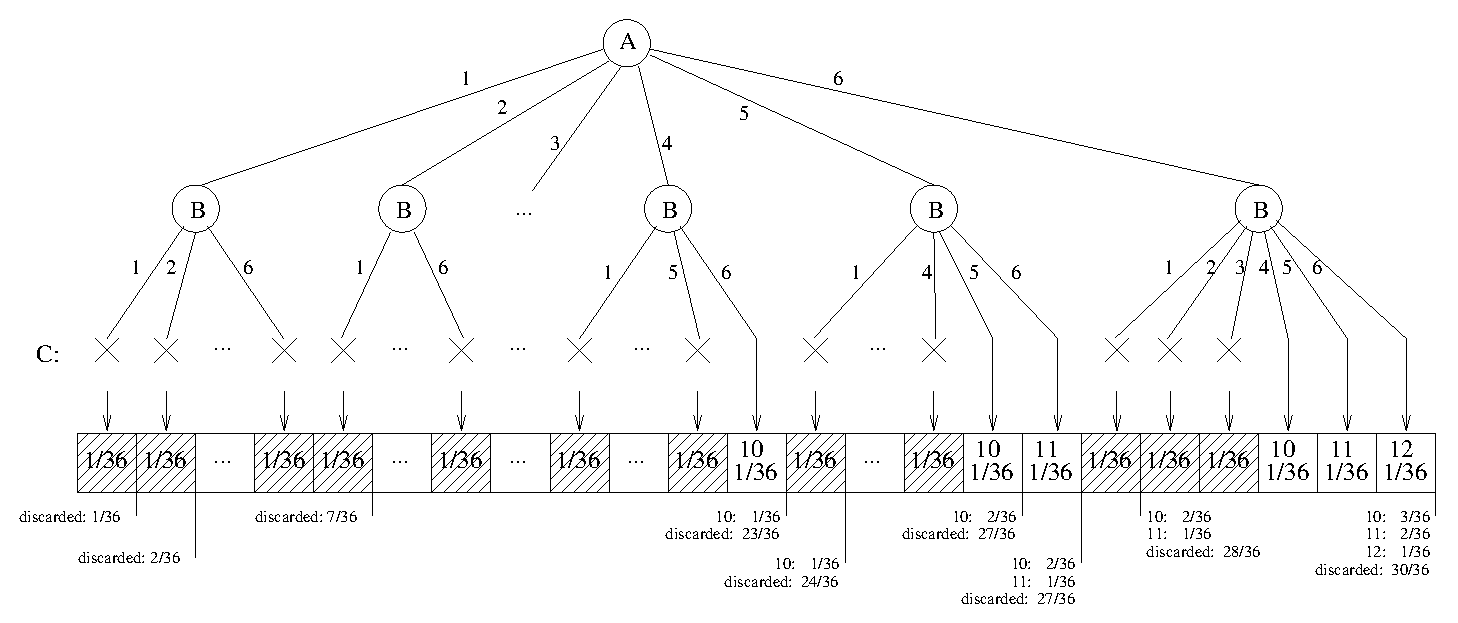
\includegraphics[width=500pt]{walkthrough.eps}
\caption{The search tree for the program in Figure~\ref{walkthrough-program}, with the corresponding possibility and impossibility stream, and contents of cache at selected points}
\label{walkthrough}
\end{figure*}

Refining the distribution in Figure~\ref{walkthrough-program} causes
Probabilistic Scheme to carry out a search through the tree in
Figure~\ref{walkthrough}.  When the \code{(roll-die)} marked \code{A}
is first encountered,\footnote{Actually, which \code{(roll-die)} is
encountered first depends on the order in which one's Scheme
implementation evaluates function arguments.  For the sake of the
exposition, I assume that function arguments are evaluated
left-to-right.} it will save its continuation and remaining options on
a search schedule, set the current density to 1/6 and return 1.  When
the \code{(roll-die)} marked \code{B} is subsequently encountered, it
will save \emph{its} continuation, current density, and remaining
options on the schedule, set the current density to $1/6 * 1/6 =
1/36$, and return 1.  From there, the evaluation will proceed
according to the standard rules of Scheme: \code{+} will compute
\code{(+ 1 1)}, \code{let} will bind \code{num} to 2, and the
\code{observe!}\ marked \code{C} will be evaluated.  Since 2 is not
greater than 9, \code{(> num 9)} will return false, and
\code{observe!}\ will abort this branch of the computation.

A failed observation translates into an impossibility in the
distribution's stream.  Since the density at the point of entry into
\code{observe!}\ was 1/36, the stream emits an impossibility that says
that 1/36 of the density is gone.  The cache records this, and if one
were to stop refining now, one would have a probability distribution
object that had a \code{min-probability} of 0 for every datum, a
\code{max-probability} of 1 for every datum, and a discarded density
of 1/36.

If one refined the distribution further, the search would resume at
the last saved point.  This means that the scheduler would remove 2
from the list of options available at \code{B}, set the current
density to $1/6 * 1/6 = 1/36$, and escape into the continuation
captured at \code{B}.  In effect, the \code{(roll-die)} marked
\code{B} would now return 2.  Then the computation would proceed as
normal: \code{+} would compute \code{(+ 1 2)}, \code{num} would get
bound to \code{3}, \code{(> 3 9)} would return \code{\#f}, and
\code{observe!}\ would fail again.  This would cause the stream to
emit another impossibility, again for density 1/36, which would get
cached, and would leave one with a probability distribution object
that had a \code{min-probability} of 0 for every datum, a
\code{max-probability} of 1 for every datum, and a discarded density
of 2/36.

With further refinement, this would continue to happen until \code{B} ran
out of saved options.  If refined beyond that point, Probabilistic Scheme will
backtrack to \code{A}.  The scheduler will remove \code{B} from the
schedule, remove 2 from the list of options remaining at \code{A}, set
the current density to $1 * 1/6 = 1/6$ (1 for the density of reaching
\code{A} and 1/6 for the density of 2 given \code{A}), and escape into
the continuation associated with \code{A}.  In other words, the
\code{(roll-die)} marked \code{A} will return 2.  Then execution
proceeds normally, so we invoke the \code{(roll-die)} marked \code{B}
again.  It will save its continuation, place its options on the
schedule, set the current density to $1/6 * 1/6 = 1/36$, and return 1.
\code{+} will compute \code{(+ 2 1)}, the \code{>} at \code{C} will
decide that 3 is still not more than 9, and the \code{observe!}\ at
\code{C} will fail again.  This will cause the stream to emit another
impossibility of density 1/36, and leave the distribution with
a discarded density of 7/36.

With yet further refinement, Probabilistic Scheme will search through all six
return values of \code{B} for \code{A} having returned 2, will
backtrack to \code{A} and have \code{A} return 3, and look through all
six of \code{B}'s options again.  The first interesting event will
occur when \code{A} returns 4 and \code{B} returns 6.  Since 4 plus 6
is 10, \code{(> 10 9)} will return \code{\#t}, and the
\code{observe!}\ will let the computation proceed.  There isn't much
computation left, so the thunk will return, and
\code{stochastic-thunk->distribution} will record a possbility whose
value is 10 and whose density is 1/36.  At this point, a total of 24/36
of the density is accounted for, leaving 12/36 unexplored.  If all 12/36
of that density went to data other than 10, then the distribution would
have 13/36 density in all, 1/36 of it allocated to 10, so the
\code{min-probability} of 10 is at this point $(1/36)/(13/36) = 1/13$.
The \code{min-probability} of all other data is still 0, as we have
not encountered them, and the \code{max-probability} of 10 is 1,
whereas the \code{max-probability} of data besides 10 is 12/13.

If we refine the distribution again, it will backtrack to \code{A}
since \code{B} is done, \code{A} will return 5, \code{B} will return
1, and \code{C} will fail.  The stream will emit another
impossibility.  The undiscovered density will decrease to 11/36, so
the \code{min-probability} of 10 will rise to $(1/36) / (12/36) = 1/12$,
and the \code{max-probability} of data other than 10 will drop to 11/12.
If we keep refining until \code{B} returns 5, then \code{C} will pass
again, and the thunk will return 10 again.  The distribution will
record the total density of 10 as 1/18.  Since at that point 7/36 of
the density is still not accounted for, the \code{min-probability} of
10 is now $2/36 / (2/36 + 7/36) = 2/9$, whereas its
\code{max-probability} is still 1.  The \code{min-probability} of
other data is still 0, but their \code{max-probability} now decreases
to 7/9.

If we refine the distribution again, \code{B} will next return 6,
\code{let} will bing \code{num} to 11, and the \code{observe!}\ at
\code{C} will pass again, allowing the stream to emit a possibility
signalling density 1/36 for the datum 11.  The \code{min-probability}
of 10 remains 2/9, the \code{min-probability} of 11 becomes 1/9, but
the \code{max-probability} of 10 is now less than 1, because the
distribution knows that some density went to 11.  Specifically, if all
6/36 of the remaining density went to 10, its density would be 8/36
out of 9/36, so the \code{max-probability} of 10 is now 8/9 (whereas the
\code{max-probability} of 11 is 7/9, and the \code{max-probability}
of other data is 6/9).

If we refine the distribution again, Probabilistic Scheme will
backtrack to \code{A} again, \code{A} will now return 6,
\code{B} will return 1, \code{C} will note that 7 is less than 9,
and the stream will emit another impossibility of density 1/36.
Less density now remains unaccounted for, so the \code{min-probability}
of each of 10 and 11 rise (to 2/8 and 1/8, respectively) and their 
\code{max-probability} fall (to 7/8 and 6/8, respectively).  The
\code{max-probability} of unseen data falls to 5/8.

Further refining will yield two more impossibilities, and then three
possibilities, for 10, 11, and 12.  The answer, in the end, is that
the probability of 10 is $(3/36) / (6/36) = 1/2$, of 11 is 1/3, of 12
is 1/6, and of all other data is 0.  If we try to refine the
distribution beyond that, the scheduler will try to backtrack past
\code{A} and note that nothing remains on the schedule.  The stream
will therefore emit the empty stream, and nothing will change.

\section{Examples}
\label{examples}

For our second example, consider the definitions in
Figure~\ref{geometric}.  The \code{geometric-select} function will
return some integer greater than or equal to \code{start}, implicitly
distributed according to a geometrically receding distribution
parametrized by \code{alpha}.  Limitations of time and computer memory
aside, this distribution is infinite, but the lazy nature of the
implementation permits 
\code{stochastic-thunk->distribution} to return a perfectly good
distribution object.  One could then call \code{distribution/refine!}\
on it until satisfaction, and \code{distribution/min-probability}
would tell one that 0 has probability at least 1/4 in this
distribution.  The upper bound, returned by
\code{distribution/max-probability}, would decrease as one refined the
distribution further and further, tending to 1/4 in the limit.

\begin{figure}[tbhp]
\begin{verbatim}
(define (geometric-select alpha start)
  (discrete-select
   (start alpha)
   ((geometric-select alpha (+ start 1))
    (- 1 alpha))))

(define receding-distribution
  (stochastic-thunk->distribution
   (lambda () (geometric-select 1/4 0))))
\end{verbatim}
\caption{A recursive definition of an infinite distribution}
\label{geometric}
\end{figure}

The infinite nature of the distribution does no harm to compositional
operations either.  For instance, one could require that the 
integers be odd either explicitly with
\begin{verbatim}
(conditional-distribution
 receding-distribution odd?)
\end{verbatim}
or implicitly with 
\begin{verbatim}
(let ((number (geometric-select 1/4 0)))
  (observe! (odd? number))
  ...)
\end{verbatim}
In this situation, the \code{min-probability} of 0 would remain 0
forever, because it is ruled out by the predicate \code{odd?}, and
both the \code{min} and \code{max} probabilities of 1 would tend, as
they should, to 7/16, from below and above, respectively, as one
refined the resulting distribution further.

The fun doesn't end there!
Figures~\ref{geom-list},~\ref{list-list}~and~\ref{tree} exemplify
definitions of distributions over arbitrary, structured objects.
\begin{figure}[tbph]
\begin{verbatim}
(stochastic-thunk->distribution
 (lambda ()
  (make-list (geometric-select 1/4 0) 'a)))
\end{verbatim}
\caption{A distribution over lists whose elements are references to
the symbol \code{a}, and whose lengths are distributed according to
the geometric distribution.}
\label{geom-list}
\end{figure}
\begin{figure}[tbph]
\begin{verbatim}
(stochastic-thunk->distribution
 (lambda ()
  (map (lambda (ignore)
        (let ((size (geometric-select 1/4 0)))
          (observe! (odd? size))
          (make-list size 'a)))
       (make-list (geometric-select 1/2 0)))))
\end{verbatim}
\caption{A distribution over lists of lists, all of unbounded lengths,
with the inner lists constrained to have an odd number of elements.}
\label{list-list}
\end{figure}
\begin{figure*}[tbph]
\begin{verbatim}
(define (tree-structure alpha)
  (discrete-select
   ('() alpha)
   ((cons (tree-structure alpha) (tree-structure alpha)) (- 1 alpha))))

(stochastic-thunk->distribution (lambda () (tree-structure 1/3)))
\end{verbatim}
\caption{A recursive distribution over tree structures.}
\label{tree}
\end{figure*}

\section{Discussion and Future Work}
\label{discussion}

This work has shown how to offer an interface for embedding
probabilistic modeling into a full, practical programming language.
Probabilistic Scheme is a proof-of-concept implementation
demonstrating that this interface is reasonable, and does not require
the creation of new programming languages from scratch.

There remain plenty of questions whose answers will help make
this system more practically useful:
\begin{itemize}
\item How useful is searching possibilities best-first,
and how could the language empower the user to supply search heuristics?
\item Numerical roundoff error\footnote{Which is probably preferable to
the denominator explosion that plagues exact rational arithmetic}
is important since extremely small
numbers are known to arise in the practice of probabilistic modeling.
What are the right techniques for dealing with it?
\item Is it possible to discover no-good sets of discrete selections and avoid
them in some dependency directed manner,
e.g.~\cite{bacchus03value},~\cite{stallman-sussman-reasoning}?
\item What are the right decision-theoretic constructs that naturally
refine distributions only as far as is useful?
\item Can Probabilistic Scheme be extended to continuous probability
distributions?
\item Can Probabilistic Scheme be extended to reasoning over
first-order and other more general propositions, rather than just
distributions?
\end{itemize}

\section{Acknowledgments}

The author would like to thank Yu-hsin Chen and Taylor Campbell for
assistance with the implementation; the anonymous reviewers for their
feedback; and Gregory Marton, Brian Milch, Gerald Sussman, Rebecca
Frankel, Tanya Khovanova, and Boris Katz for many useful discussions.

\begin{thebibliography}{10}

\bibitem{sicp}
H.~Abelson, G.~J. Sussman, and J.~Sussman.
\newblock {\em Structure and Interpretation of Computer Programs}.
\newblock MIT Press, 1984.

\bibitem{bacchus03value}
F.~Bacchus, S.~Dalmao, and T.~Pitassi.
\newblock Value elimination: Bayesian inference via backtracking search, 2003.

\bibitem{friedman1999lpr}
N.~Friedman, L.~Getoor, D.~Koller, and A.~Pfeffer.
\newblock {Learning probabilistic relational models}.
\newblock {\em Proceedings of the Sixteenth International Joint Conference on
  Artificial Intelligence}, pages 1300--1309, 1999.

\bibitem{kelsey1998rra}
R.~Kelsey, W.~Clinger, J.~Rees, et~al.
\newblock {Revised5 Report on the Algorithmic Language Scheme}.
\newblock {\em SIGPLAN Notices}, 33(9):26--76, 1998.

\bibitem{koller1998pfb}
D.~Koller and A.~Pfeffer.
\newblock {Probabilistic frame-based systems}.
\newblock {\em Proc. AAAI}, 98, 1998.

\bibitem{mccarthy1963bmt}
J.~McCarthy.
\newblock {A Basis for a Mathematical Theory of Computation}.
\newblock In P.~Braffort and D.~Hirschberg, editors, {\em Computer Programming
  and Formal Systems}. North-Holland, Amsterdam, 1963.

\vfill\eject
\bibitem{milch2005bpm}
B.~Milch, B.~Marthi, S.~Russell, D.~Sontag, D.~Ong, and A.~Kolobov.
\newblock {BLOG: Probabilistic models with unknown objects}.
\newblock {\em Proceedings of the Nineteenth Joint Conference on Artificial
  Intelligence}, 2005.

\bibitem{pfeffer01ibal}
A.~Pfeffer.
\newblock {IBAL}: A probabilistic rational programming language.
\newblock In {\em {IJCAI}}, pages 733--740, 2001.

\bibitem{ramsey2002slc}
N.~Ramsey and A.~Pfeffer.
\newblock {Stochastic lambda calculus and monads of probability distributions}.
\newblock {\em Proceedings of the 29th ACM SIGPLAN-SIGACT symposium on
  Principles of programming languages}, pages 154--165, 2002.

\bibitem{russell1995aim}
S.~Russell and P.~Norvig.
\newblock {\em {Artificial intelligence: a modern approach}}.
\newblock Prentice-Hall, Inc. Upper Saddle River, NJ, USA, 1995.

\bibitem{sahami1998baf}
M.~Sahami, S.~Dumais, D.~Heckerman, and E.~Horvitz.
\newblock {A Bayesian approach to filtering junk e-mail}.
\newblock {\em Learning for Text Categorization: Papers from the 1998
  Workshop}, 62, 1998.

\bibitem{segal2001rpm}
E.~Segal, B.~Taskar, A.~Gasch, N.~Friedman, and D.~Koller.
\newblock {Rich probabilistic models for gene expression}.
\newblock {\em Bioinformatics}, 17(Suppl 1):S243--52, 2001.

\bibitem{spiegelhalter1994bbi}
D.~Spiegelhalter, A.~Thomas, N.~Best, and W.~Gilks.
\newblock {BUGS: Bayesian inference using Gibbs sampling}.
\newblock {\em MRC Biostatistics Unit, Cambridge, England. www. mrc-bsu. cam.
  ac. uk/bugs}, 1994.

\bibitem{stallman-sussman-reasoning}
R.~M. Stallman and G.~J. Sussman.
\newblock Forward reasoning and dependency directed backtracking in a system
  for computer-aided circuit analysis.
\newblock AI Memo 380, MIT Artificial Intelligence Laboratory, September 1976.

\bibitem{thrun2006pta}
S.~Thrun, M.~Montemerlo, and A.~Aron.
\newblock {Probabilistic Terrain Analysis For High-Speed Desert Driving}.
\newblock {\em Proc. Robotics Science and Systems, Philadelphia, PA, USA,
  August}, pages 16--19, 2006.

\end{thebibliography}

%\bibliographystyle{abbrv}
%\bibliography{probscheme}

\end{document}
